\section{Proposed Research}
\label{sec:proposed-work}

\subsection{Specific Aim 1: Membrane vesicles as self-organized granules}
\label{sec:specificaim1}
We introduced \eqref{eq:RBT}--\eqref{eqn:stressbalance} to complement
existing methods for studing vesicles and bilayers. The simulation
results in (Figures~\ref{fig:JPv_linearshear} and~\ref{fig:JPv_rupture})
show that two-dimensional, granule-based vesicles replicate the
equilibria and hydrodynamics for continuous curves~\cite{FuQuRyYo22,
Fu2018_SIAM}. Our next goal is to study the model using rigorous
analysis and consider three-dimensionsional effects. 

The first step is to obtain some solid well-posedness results for
\eqref{eq:RBT}--\eqref{eqn:stressbalance}. This system is an autonomous
ordinary differential equation for the body transformations $F_i$ with
the rate of change defined by a system of PDEs. Regarding this system,
in the single-well case and for fixed $t$, the linear system has a
unique solution ($\phi, \uu$) under appropriate assumptions for the
boundaries and boundary data~\cite{manasthesis, rac-gre2016, LAX}. These
define the instantaneous rigid body translational velocity and rotation.
This leads to 
\begin{quotation}
  \noindent
  \textbf{Problem 1.} 
  Consider a collection the closed, disjoint granules $U_i$ with smooth
  boundary, with no-slip, rigid body motion boundary conditions, and a
  linear background flow. Assume a single-well potential and a smooth
  phase field boundary condition. What is the well-posedness in time of
  the coupled system \eqref{eq:RBT}--\eqref{eqn:stressbalance}?
\end{quotation}
Problem 1 involves mathematically interesting techniques. First, we
must establish that the system has a local-in-time solution. This
involves domain perturbations and estimates for the solutions of second
order elliptic equations~\cite{Savar2002DomainPA, DANERS20081,
Lamboley2015EstimatesOF}, which also find extensive application in
extremal domain problems~\cite{Schiffer1954VariationOD,
Henrot2006ExtremumPF, bogosel:hal-03607776,Bogosel2022OnTP}, for
example. For global-in-time solutions, we can ensure positivity in time
for the distance between granules using lubrication
forces~\cite{cawthorn_balmforth_2010, leal_2007}. Finally, we can
describe the granule-flow behavior in the zero-screening length limit.
In this limit, we should recover the hydrodynamics of a (noninteracting)
rigid body suspension. 

In the double-well potential case,equation~\eqref{eqn:phase} is a
nonlinear Allen-Cahn equation. This situation models granules immersed
in a two-phase fluid (e.g.~granules in an emulsion) where there is an
interesting interplay between the long-range alignment of granules and
the diffusive interface energy of the free boundary between fluid
phases. On unbounded domains like $\Omega(t)$, Allen-Cahn equations can
have multiple solutions~\cite{Alama1997StationaryLS,
Alikakos2008OnAE, Bronsard1993OnTB, Byeon2014SolutionsOH, Byeon2013OnAP,
Alessio2005ENTIRESI, Trumper2007ExistenceOA, Benci2019MultipleSF} and so
we must reformulate~\eqref{eqn:phase}. A natural modification changes
\eqref{eqn:phase} to an initial value problem with transport by the
background fluid;
\begin{align}
  \label{eqn:phase_transport}
  \phi_t + \uu \cdot \nabla
  = -\beta \frac{\delta E}{\delta \phi}
  = \beta(\epsilon^2 \Delta \phi - W'(\phi)),
  \quad \phi(\xx,0) = \phi_0(\xx),
\end{align}
for initial data $\phi_0$. The modified system enjoys an energy law
similar to~\eqref{eq:energy_law} with an addtional dissipation term
involving the square the Euler-Lagrange derivative $\frac{\delta
E}{\delta \phi}$ and dampening factor $\beta > 0$. There are several
works dealing with the characterization of the geometric evolution of
interfaces under the Allen-Cahn and Cahn-Hilliard
equations~\cite{Christlieb2019CompetitionAC, Gavish2011CurvatureDF,
Dai2019WeakSF, Promislow2017ExistenceBA, Dai2015CompetitiveGE,
Promislow2012CriticalPO, Dai2022GeometricEO, Dai2020MinimizersFT,
Dai2013GeometricEO, Promislow2022UndulatedBI} and well-posedness when
coupled to flow in static domains~\cite{Jiang2017TwophaseIF,
Liu2012StrongSF, Giorgini2019WellPosednessOA, Wu2022WellposednessOA,
Gal2010AsymptoticBO, Giorgini2020DiffuseIM, Giorgini2019UniquenessAR}.
The proposed research extends these results to problems with moving
domains. A closely related and strongly developing direction in the area
of nematics liquid crystals concerns the interaction of Landau de Gennes
functionals with colloids, and studies the qualitative structure of
defects around single or multiple coloidal
particles~\cite{doi:10.1098/rsta.2020.0432, Alama2015MinimizersOT,
Alama2021SaturnRD, PhysRevE.96.042702}. PI Ryham has several works on
membrane vesicles dealing both with Allen-Cahn formulations and
fluid-vesicle interactions~\cite{QiangDu09, RYHAM20112929, RyCoEi12,
Ryham2017OnTV}.

The second problem considers the approximation of elastic energy of
curves and surfaces, and seeks to make rigorous the simulation results
of~\cite{FuQuRyYo22, Fu2018_SIAM}. We employ the so-called
``amphiphilic'' boundary condition that leads to a collection of
granules that form bilayers. Referring to
Figure~\ref{fig:amphiphilic_assembly}, 
\begin{align}
\label{eq:amphiphilic_BC}
  \phi(\xx) = h_i(\xx) = \tfrac{1}{2}\left(\dd_i \cdot 
    (\xx - \aa_i)/c_i + 1\right), \quad \xx \in \Gamma_i,
\end{align}
where $\dd_i$ is the director, $\aa_i$ is the center, and $c_i$ the
``radius'' of the $i$th granule. The phase $\phi$ takes values close to
$1$ on in the direction $\dd_i$, representing a hydrophobic tail, and
values close to $0$ in the direction $\dd_i$ representing the
hydrophilic head.

\begin{quotation}
  \noindent
  \textbf{Problem 2.}
  Consider a collection of two-dimensional amphiphilic granules along a
  closed curve $\mathbf{C}$. What is the sharp interface limit of the
  energy $E$ as the number of granules goes to infinity and their size
  to zero?
\end{quotation}
The sharp interface model represents a membrane vesicle as an
inextensible continuous surface $\Sigma$ with elastic energy
\begin{align}
  \label{eq:Canham-Helfrich}
  \int_{\Sigma} k_B(H - k_0)^2\, dS,
\end{align}
where $H$ is the mean curvature, $k_0$ is a spontaneous curvature, and
$k_B$ is a bending modulus. One can also account for extensibility by
including in~\eqref{eq:Canham-Helfrich} an additional stretching term
$k_A(\alpha - \alpha_0)^2/\alpha_0^2$ where $\alpha$ and $\alpha_0$ are
the deformed and equilibrium area densitities respectively.

\begin{wrapfigure}[12]{r}{0.5\textwidth}
  \vspace{-5pt}
  \centerline{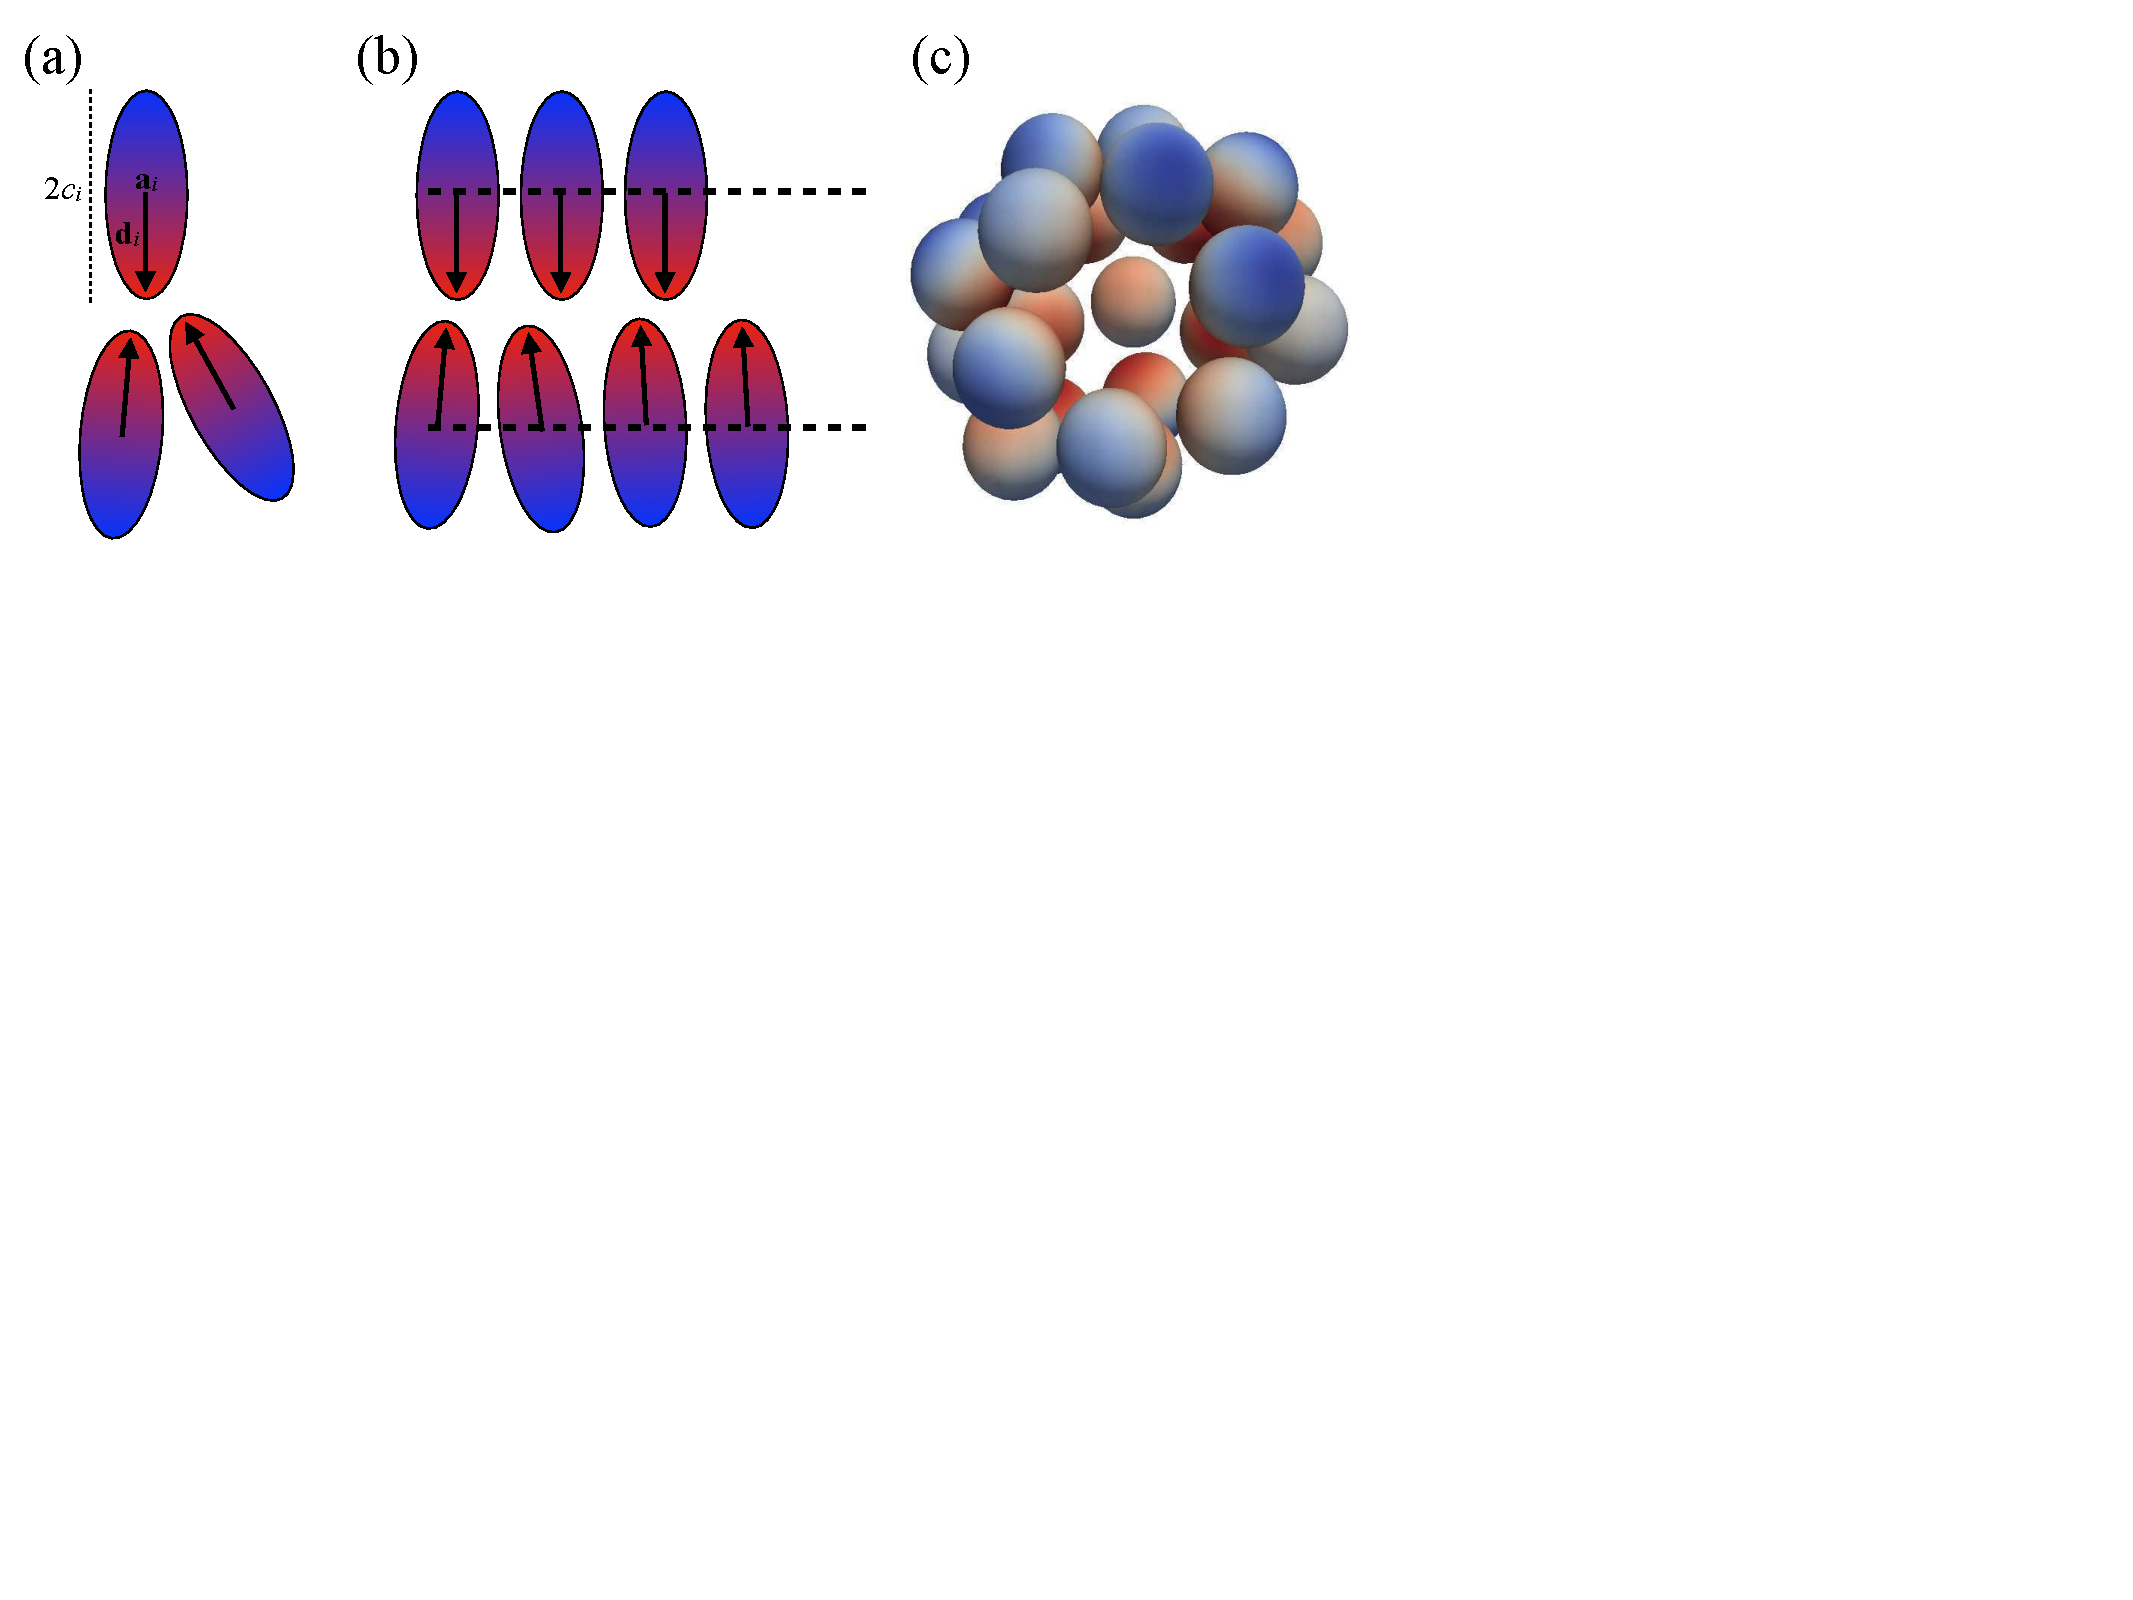
\includegraphics[width=0.5\textwidth]{figures/SA1Figures/AmphiphilicAssembly.pdf}}
  \vspace{-5pt}
  \caption{\label{fig:amphiphilic_assembly} Self-organization under
  amphiphilic boundary condition. (a) Granules first match hydrophobic
  tails (red), (b) then align length-wise. (c) The principle of
  self-organization holds in three dimensions as simulated by Kohl,
  Corona, and Veerapaneni~\cite{koh-cor-che-vee2021}.}
\end{wrapfigure}
Bending enters through the splay of the granule directors. In
Figure~\ref{fig:JPv_linearshear}, for example, the directors have
negative, respectively positive, splay $\nabla_{\Sigma} \cdot \dd$ in
the outer, respectively inner monolayers. Here $\nabla_{\Sigma}\cdot{} =
\nabla \cdot {} - \mathbf{N}\mathbf{N}^T \nabla$ is the surface
divergence for the outward unit surface normal $\NN$. From differential
geometry, we have that $\nabla\cdot \dd = \pm 2H$ whenever $\dd$ is
everywhere parallel to $\NN$, and this is how the curvature term arises
in equation~\eqref{eq:Canham-Helfrich}. For two-dimensional vesicles,
$H$ is replaced with the curvature $\kappa$ of the curve $\mathbf{C}$.
Granules are at rest when attraction balances repulsion, and will have
stretching when the distance between neighboring granules is increased
from rest.

PI Ryham has experience in the sharp interface analysis for phase field
formulations of elastic bending energy~\cite{0951-7715-18-3-016, Du05},
and topological indicators~\cite{DuEuler}, as well as for
Poisson-Boltzman equations~\cite{Lee2018, 1531-3492_2006_2_357}. Tools
for addressing Problem 2 have been developed for bulk nematic liquid
crystal potentials in the area of colloidal
homogenization~\cite{Canevari2019DesignOE, doi:10.1137/18M1163919,
doi:10.1137/18M1163919, BERLYAND200597, doi:10.1137/130910348}, and is
related to dimension reduction for curved nematics confined to thin
films~\cite{Golovaty2017DimensionRF, Golovaty2015DimensionRF,
doi:10.1142/S0218202516500470, FoFrLe07}. We start by assuming circular
granules aligned normally to the curve, and then generalize the problem
to account for aspect ratio of elliptical granules and nonzero tilt. 

Finally, to consider three-dimensionsional effects, we will generalize
Problem 2 to \emph{numerically} study the energies of amphiphilic
granules confined to surfaces. Recent work on nematics on a surface has
studied the interplay between surface geometry and a director
field~\cite{Nestler2020PropertiesOS, Nitschke2018NematicLC,
Nestler2018OrientationalOO, Nitschke2019HydrodynamicII,
Nitschke2020LiquidCO}. Researchers have formulated finite element
methods for~\cite{Bartels2012FiniteEM, Nochetto2015NumericsFL,
Nestler2019AFE} and studied minimizers~\cite{Segatti2014EquilibriumCO,
Segatti2014AnalysisOA}. On the other hand, in biophysics, researchers
have derived the general Helfrich energy for lipid bilayers that
involves effects coupling lipid tilt to director
splay~\cite{Hamm2000ElasticEO, Terzi2019CurvatureTiltTO, Terzi2019ACQ,
Terzi2017NovelTC, Pinigin2020NewCT}. This energy
contains~\eqref{eq:Canham-Helfrich} as a special case.
\begin{quotation}
  \noindent
  \textbf{Problem 3.} Simulate surfaces made up of three-dimensional,
  amphilic granules. Numerically investigate the limiting energy for
  large $N_b$ suspensions.
\end{quotation}
In his much noticed Biophysical Journal and Nature
papers~\cite{RyKlYaCo16, Chetal16}, PI Ryham calculated the least energy
path for \emph{membrane fusion} using a surface-director model based on
the general Helfrich energy. The energy barriers calculated
in~\cite{RyKlYaCo16} proved consistent with later molecular dynamics and
experimental results~\cite{SmRiMu19, 2017PNAS..114.1238F}.

The completion of Problems 1, 2, and especially 3 requires additional
algorithmic implementation including a fast summation method such as the
fast multipole method. The implementation details, in particular how we
deal with large granule numbers and three-dimensional systems are
described in Specific Aim 2 (\S\ref{sec:specificaim2}).
%\begin{equation}
%\label{eq:Helfrich}
%  \begin{aligned}
% &\int_{\Sigma}
%  %\label{eq:Pinigan}
%\tfrac{1}{2}k_{b}[(\nabla_{\Sigma} \cdot \mathbf{d} + k_{0})^{2} -  k^{2}_{0}]  
%+ \tfrac{1}{2}k_{\theta}\mathbf{T}^{2} + \tfrac{1}{2}k_a[(\alpha - \alpha_0)^2 - \alpha_0^2] \\
%&+ k_{c}\textbf{T} \cdot \nabla_{\Sigma} \nabla_{\Sigma} \cdot \mathbf{d}  + \tfrac{1}{2}k_{g}(\nabla_{\Sigma} \nabla_{\Sigma} \cdot \mathbf{d})^{2}
% + A\alpha \nabla_{\Sigma} \cdot \mathbf{d}
%+ B \mathbf{T} \cdot \nabla_{\Sigma} \alpha \\
%&- \tfrac{1}{2}k_c |\nabla_{\Sigma} \alpha|^2 + C \nabla_{\Sigma} \alpha \cdot \nabla_{\Sigma} \nabla_{\Sigma} \cdot \mathbf{d}\,dS
%\end{aligned}
%\end{equation}
%in the lipid director $\dd$,
%tilt vector $\mathbf{T}$
%the difference between the lipid director $\mathbf{d}$ and the surface normal
%$\mathbf{N}$; area per lipid $\alpha$,
%and where $\nabla$ and $\nabla \cdot$ are the surface gradient and surface divergence, respectively. 
%The two models \eqref{eq:Canham-Helfrich} and \eqref{eq:Helfrich} agree
%when $\mathbf{T} = 0$ and $\alpha = \alpha_0$ everywhere.
%The remaining term $k_B$, $k_{\theta}$, $k_a$, $k_c$, $k_g$, $A$, $B$, $C$ are
%appropriate elastic moduli.




